\documentclass{article}
\usepackage[utf8]{inputenc}
\usepackage{pdfpages}
\usepackage{amsmath}
\usepackage{bm}
\usepackage{hyperref}
\usepackage{enumitem}
\usepackage{graphicx}
\usepackage[margin=1in]{geometry}
\usepackage{float}
\usepackage{subfigure}
\usepackage{chngcntr}
\counterwithin{figure}{section}
\graphicspath{ {images/} }
\title{RBE/CS549 Project: Boat Tracking/Detection}
\author{Jordan Burklund \and James Kuszmaul}
\begin{document}
\maketitle

We are currently working on a robotic sailboat for the
International Robotic Sailing Competition (\url{http://sailbot.org}). For this,
we have several days of GoPro footage collected from the prow of Professor
Michalson's motorboat, which we used for developing these algorithms.

\section{General Approach}

Overall, the object pipeline is as follows:
\begin{figure}[H]
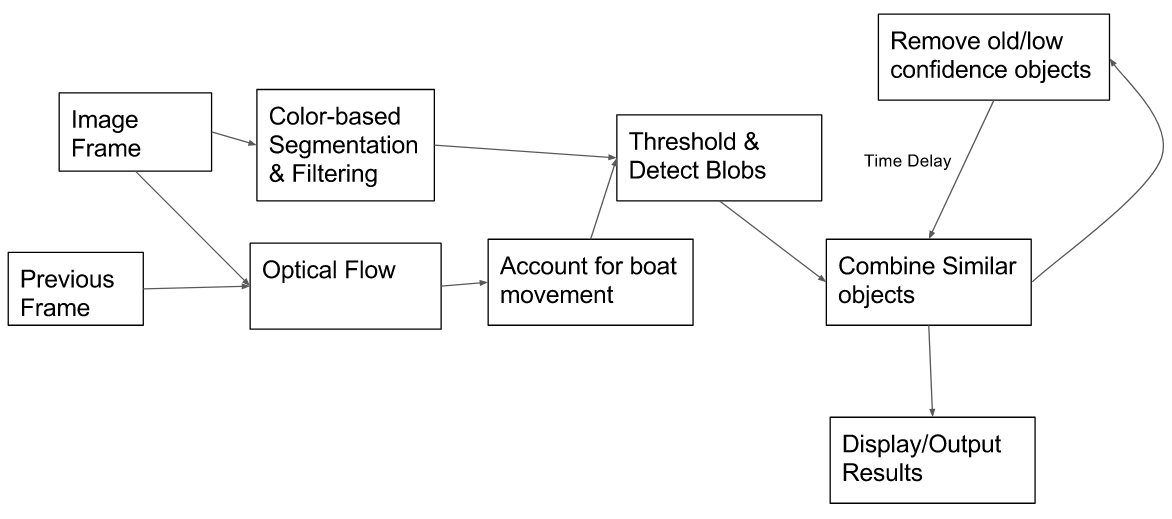
\includegraphics[width=16cm]{algorithm_flowchart}
\centering
\caption{High-Level Image Processing Pipeline}
\end{figure}


\begin{enumerate}
\item We read a frame of video and convert it to HSV space
\item Perform a slew of static transforms to try and determine,
      based on the content of a single frame, which areas are and
      are not water/sky/land/objects (see Figure \ref{fig:boatconf}:
  \begin{enumerate}
    \item We use a nonlinear k-means classification to
          identify non-water based areas
    \item And then use Matlab's \texttt{bwareaopen} to
          identify the connected areas of the sky
  \end{enumerate}
\item Use optical flow information from a given pair of frames to
      locate the moving objects in a frame, based on Matlab's
      \texttt{opticalFlowFarneback}, and a simple model of the
      expected flow of the water to filter out the background in
      the optical flow space, resulting in confidence scores
      as in Figure \ref{fig:diff_magnitude}
\item Combine the above to determine a set of viable blobs using erodes/dilates
      and Matlab's \texttt{bwlabel}
\item Associate the blobs with each other and with preexisting objects,
      creating new objects for blobs that can't be associated with any
      preexisting objects, based on:
  \begin{enumerate}
    \item Similarity in blob/object velocities
    \item Similarity of blob/object position
    \item Taking weighted averages of velocities to combine them, and
          combining the object bounding boxes
  \end{enumerate}
\item Update objects in preparation for the next frame, updating
      positions using velocities, reducing and increasing confidence
      scores as appropriate, deleting objects with sufficiently low
      scores
\end{enumerate}

\begin{figure}[H]
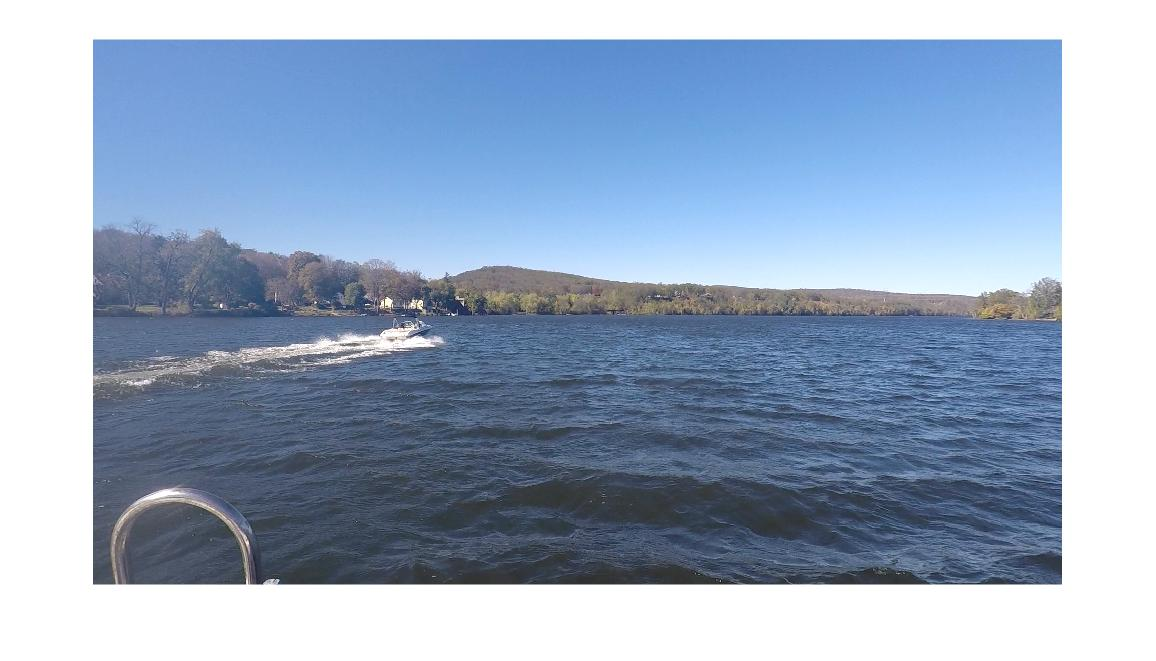
\includegraphics[width=7.8cm]{hsv_kmeans2_orig}
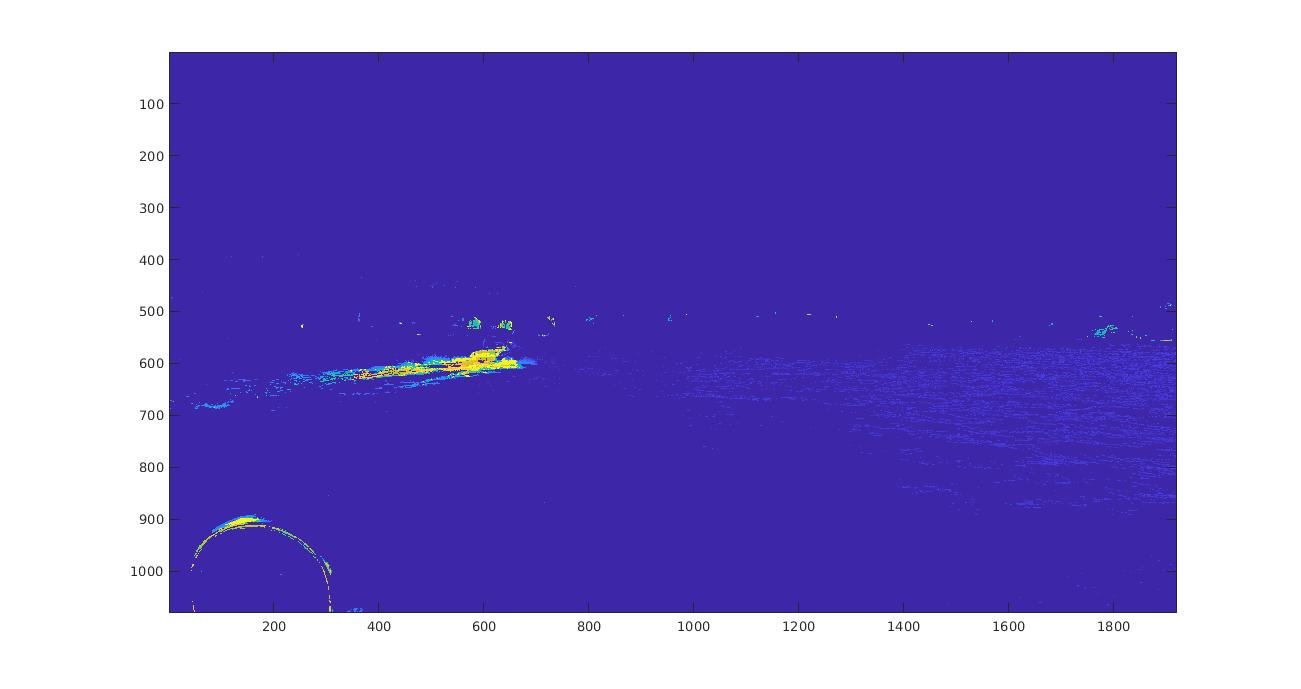
\includegraphics[width=8.5cm]{hsv_kmeans2_suppressed}
\centering
\caption{Boat Confidence Results}
\label{fig:boatconf}
\end{figure}

\begin{figure}
\centering
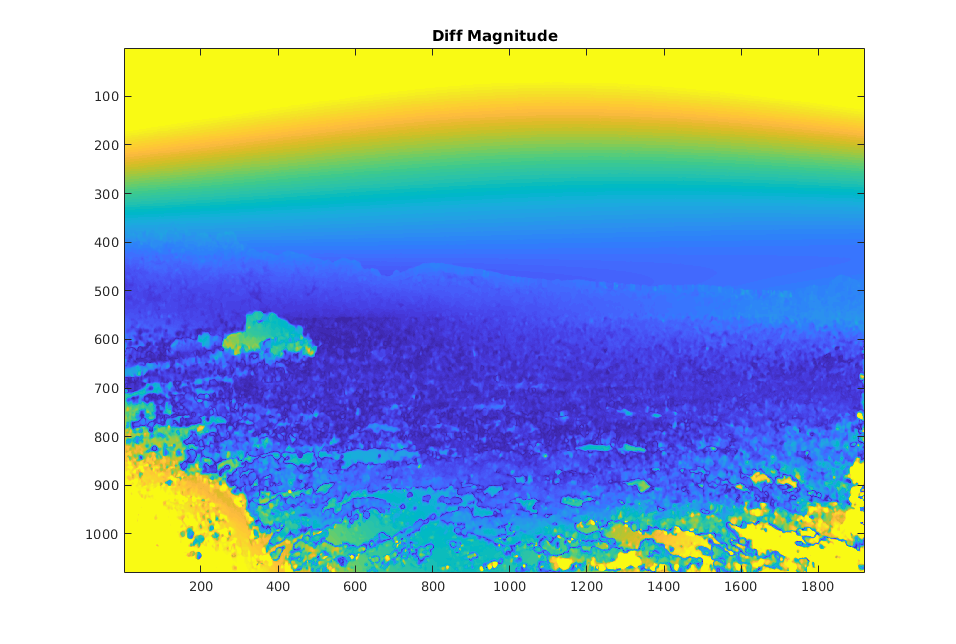
\includegraphics[width=0.6\textwidth]{diff_magnitude}
\caption{Difference between the measured and modelled optical flow.
         Dark blue means perfect match, bright yellow means a poor match (and
         higher likelihood of an object).
         The sky is later filtered out by ignoring that half of the image.}
\label{fig:diff_magnitude}
\end{figure}

\begin{figure}
\hfill
\subfigure[Blobs pre-filtering]{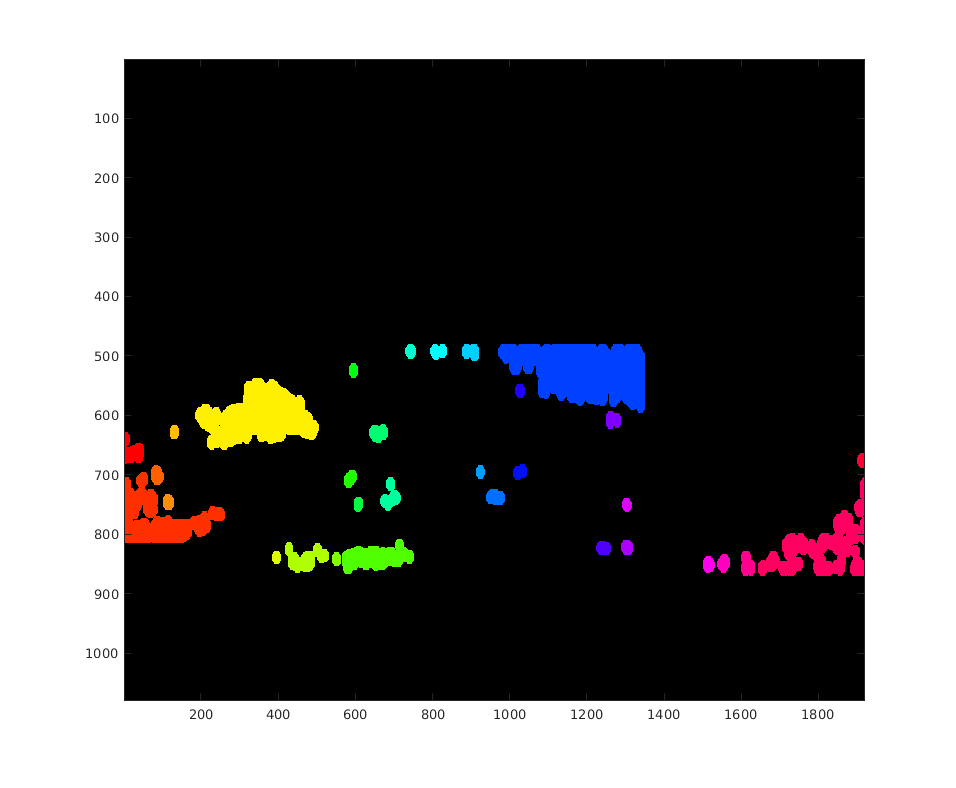
\includegraphics[width=0.3\textwidth]{threshold_bwlabel}}
\hfill
\subfigure[Blobs
post-filtering]{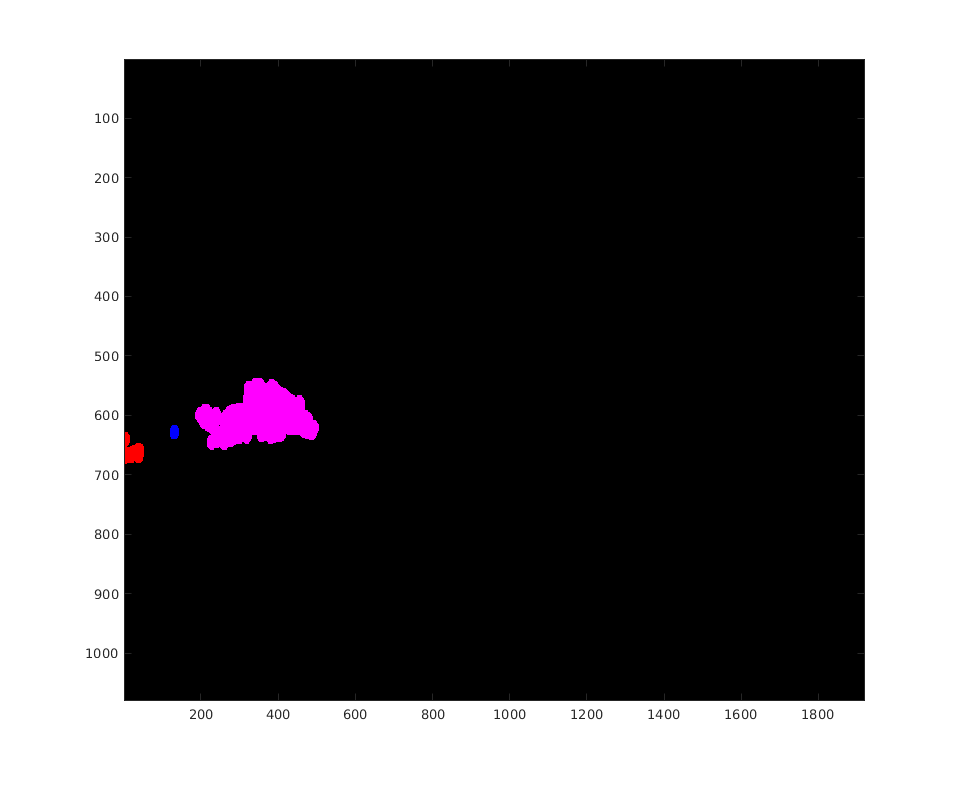
\includegraphics[width=0.3\textwidth]{filtered_labels}}
\hfill
\caption{Results of blob detection on HSV and optical flow confidences}
\label{fig:blobs}
\end{figure}

\section{Results}

\begin{figure}
\centering
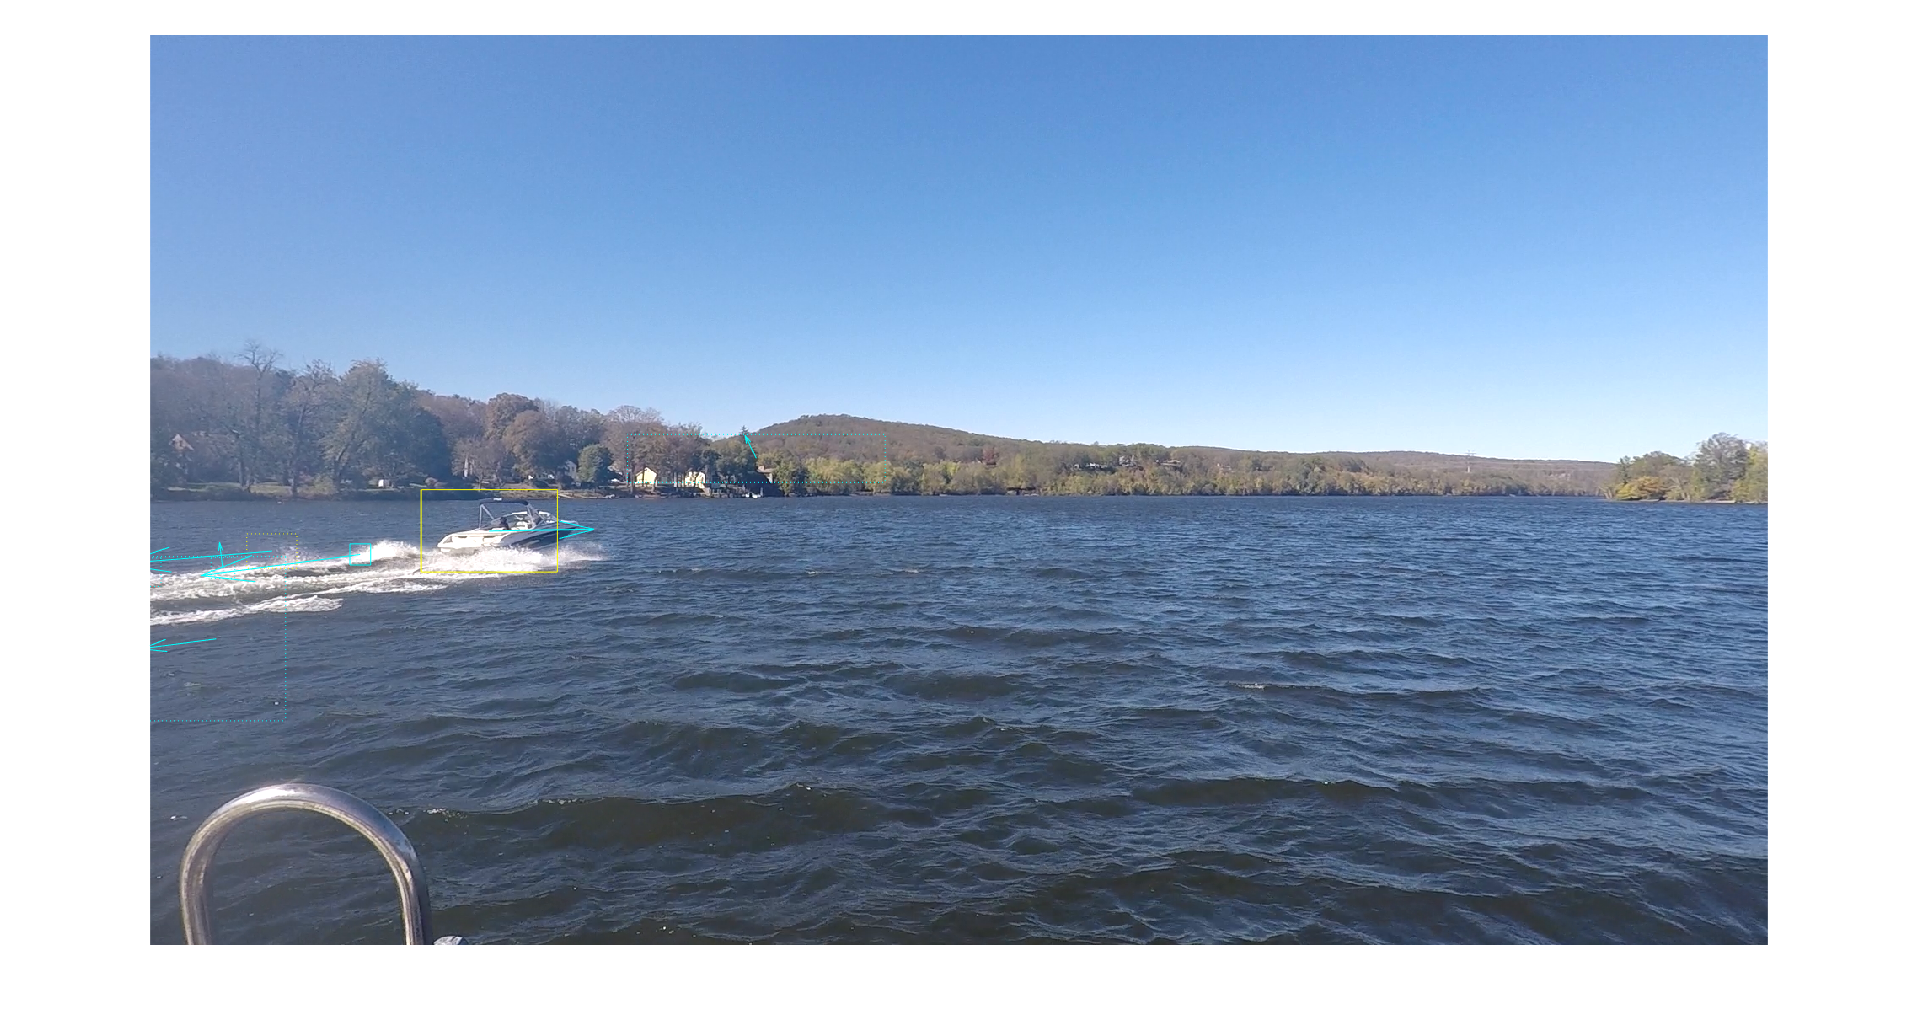
\includegraphics[width=0.5\textwidth]{example_detection}
\caption{Sample frame of the whole stack running}
\label{fig:example_detection}
\end{figure}

In Figure \ref{fig:example_detection}, we see an individual frame from the
algorithm, where we have:
\begin{itemize}
\item The boat identified by a yellow (indicating that it has existed for at
      least 10 frames) solid (indicating high confidence) box with an arrow
      pointing leftwards, roughly in the direction of its movement.
\item Several solid and dashed boxes detecting the wake of the boat.
\end{itemize}

Longer videos can be found in our presentation:

\begin{description}
\item[\url{https://drive.google.com/file/d/1FoKWkp5xDSKwp5YyluKrclo_kGFU4gsg/view?usp=sharing}]
  In this video we have a longer view of the same boat as Figure
  \ref{fig:example_detection}
\item[\url{https://drive.google.com/file/d/1ndVSwF77_4va6U8rWT4FGJOXq1AjKL_Z/view?usp=sharing}]
  This has a slightly shorter capture of a different boat, indicating some
  degree of robustness to different individual instances
  \ref{fig:example_detection}
\end{description}

For runtime (as we hope to run these algorithms on a boat in real time),
we currently are looking at around 3 seconds per frame, running single-threaded
on a laptop CPU. Given reasonable optimizations, lower resolutions, and lower
frame-rates, we can likely get these times down to work onboard the boat.

\section{Future Work}

For future work, we need to actually improve the timing (as mentioned above) to
work in real time, improve robustness for a greater variety of conditions
(including different weather), and
to increase the generality to function on a less stable platform---our boat will
certainly be pitching and rolling substantially more than the platform we had
for this footage.

\end{document}
